\section{Bloc mémoire}

\indent Cette première partie traite de la génération du bloc mémoire fonctionnel.
L'objectif est d'obtenir un bloc contenant un nombre générique de mémoires ainsi qu'un décodeur pour en gérer l'accès, via des signaux \textit{Chip Select}. \\
\indent Comme indiqué lors de l'introduction, pour chaque sous module du bloc mémoire, des bancs de test ont été réalisé grâce à Cocotb, \textit{"COroutine based COsimulation TestBench"}, un environnement de vérification VHDL et SystemVerilog basé sur le langage Python.
C'est un outil open source que nous avons couplé à ghdl pour la compilation du VHDL et à gtkwave pour afficher les résultats.
Il a été spécifiquement pensé pour réduire le temps d'écriture de bancs de tests et prône la réutilisation de designs, philosophie appropriée pour le module ME2.

\subsection{Récupération d'une IP de RAM}

\indent Il nous a été fourni un modèle simple de mémoire RAM.
La première tache vise à comprendre son fonctionnement puis à trouver une solution afin de rendre son implémentation générique tant sur la taille des données que sur l'adresse.
Le modèle récupéré génère une RAM par un tableau de vecteurs d'une taille variable selon la taille du bus d'adresses.

\begin{figure}[h]
	\centering
	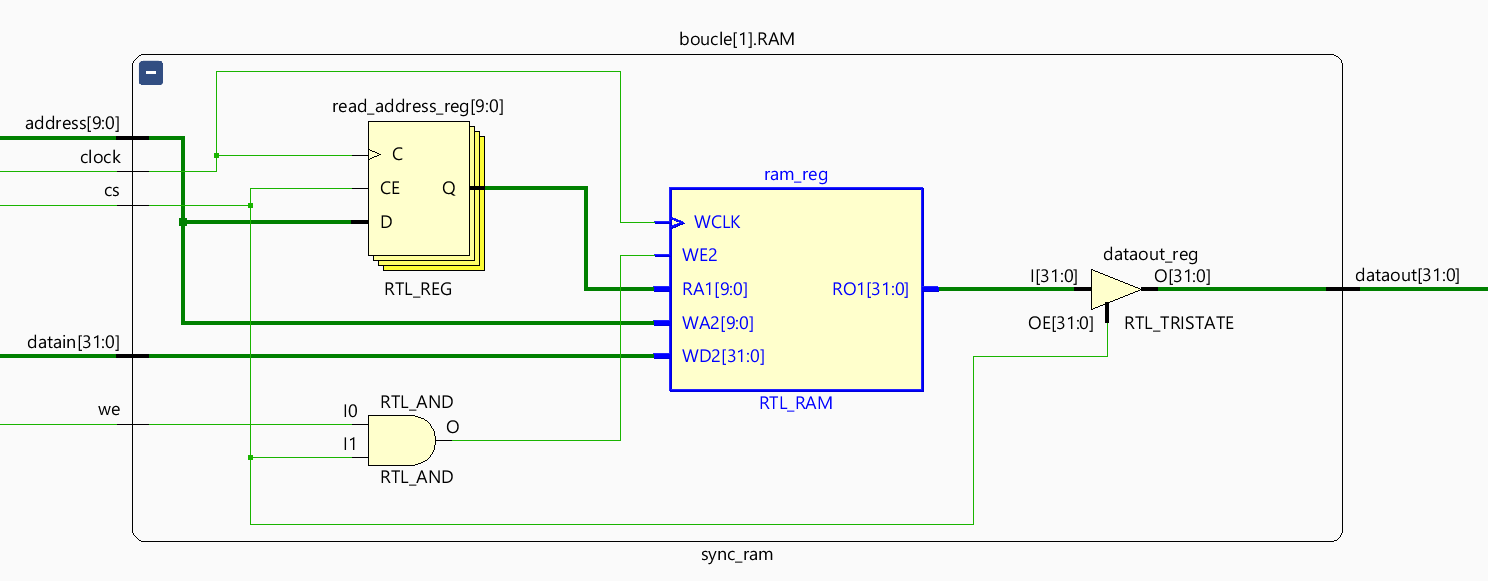
\includegraphics[width=0.97\linewidth]{bloc_ram.png}
	\caption{Bloc RAM niveau RTL}
	\label{fig:synth_bloc_ram}
\end{figure}

\indent Après modification du modèle, la lecture et l'écriture sur le bus de données en sortie n'ont lieu que lorsque le signal \textit{Chip Select (cs)} est à l'état haut.
Nous avons pu générer un banc de test avec Cocotb qui consistent à tester l'écriture via le signal \textit{Write Enable (we)} et l'activation selon le signal \textit{cs}.

\begin{figure}[h]
	\centering
	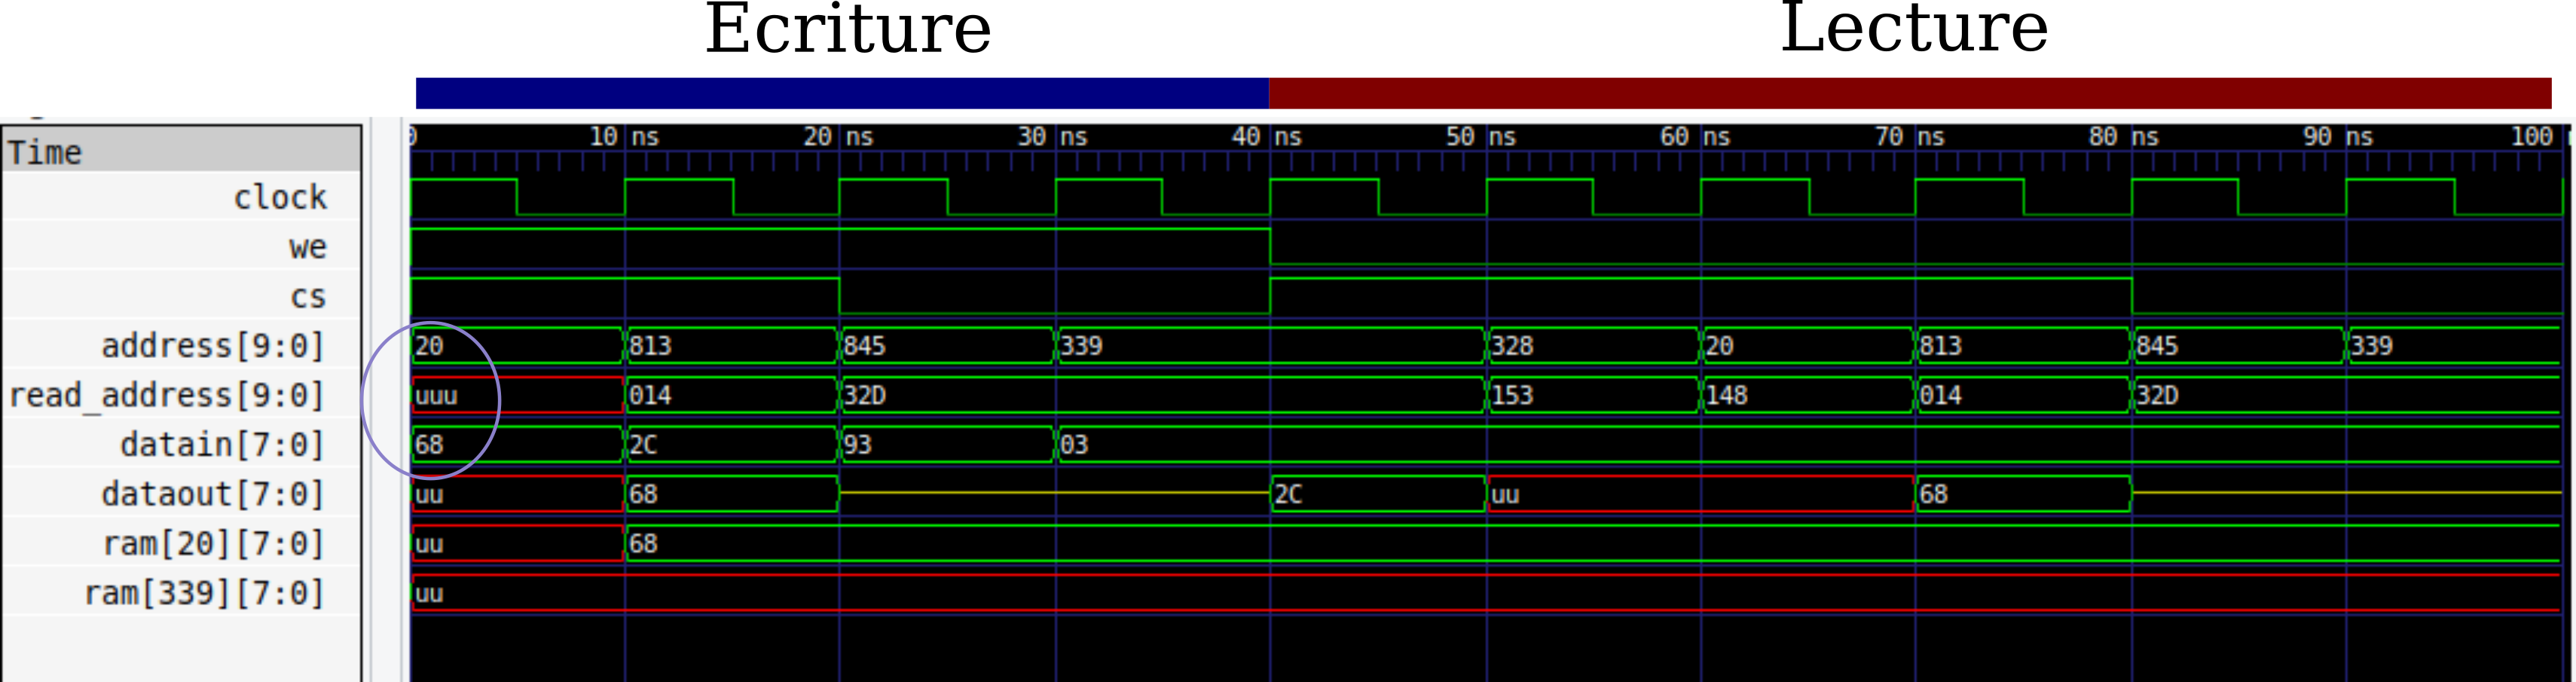
\includegraphics[width=0.97\linewidth]{ramchip_wave.draw.png}
	\caption{Simulation du bloc mémoire}
	\label{fig:wave_bloc_ram}
\end{figure}

\indent Sur la figure ci-dessus, nous pouvons vérifier le comportement de la mémoire.
Dans un premier temps, des valeurs sont écrites en mémoire (\textit{we} = 1) avec des variations du signal \textit{cs} pour vérifier si les écritures ont lieu ou non.
Dans un deuxième temps, des cycles de lecture s'enchaînent aux mêmes adresses pour vérifier le contenu de la RAM.
En jouant également sur la valeur du signal \textit{cs}, nous pouvons voir que la sortie est indéfinie lorsque \textit{cs} = 0, que la valeur contenue en adresse 20 de la RAM est correctement lue, et que l'adress 339 est indéfinie puisque \textit{cs} n'était pas actif lors de l'écriture.

\subsection{Décodeur d'adresse}

\indent En vue de pouvoir intégrer plusieurs instances de la RAM, il est nécessaire de décrire un décodeur d'adresses qui analysera les n-bits de poids fort (n pour la généricité) pour accéder aux différentes RAM en lecture ou en écriture.

\begin{figure}[h]
	\centering
	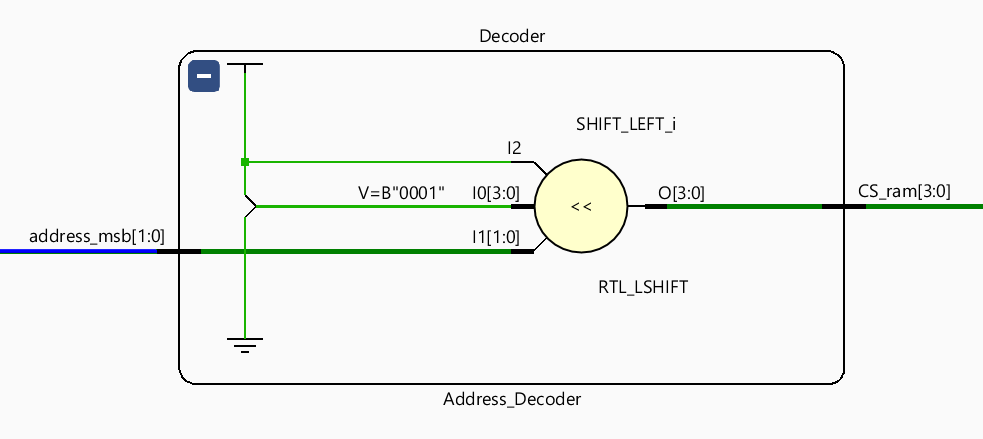
\includegraphics[width=0.97\linewidth]{decodeur.png}
	\caption{Décodeur au niveau RTL}
	\label{fig:synth_bloc_decodeur}
\end{figure}

\indent Le décodeur fonctionne de façon purement combinatoire : le fonctionnement interne est simplement un décalage à gauche d'un bus de taille $ 2^{n} $ et de valeur initiale 1; le nombre de décalages effectués est égal à la valeur des bits d'entrée et il y a $ 2^{n} $ valeurs possibles.
Le banc de test est élémentaire : il suffit de tester les $ 2^{n} $ entrées possibles, n étant le nombre de bits de poids fort pris en considération. Via l'utilisation de Cocotb, il est aisé de vérifier les sorties pour des n différents (ci-dessous, les tests pour n = 2 et n = 3).

\begin{figure}[h]
	\centering
	\begin{subfigure}{0.3\textwidth}
		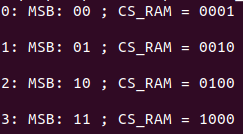
\includegraphics[width=\textwidth]{decoder_entry_2_out.png} 
	\end{subfigure}
	\, \, \, \,
	\begin{subfigure}{0.3\textwidth}
		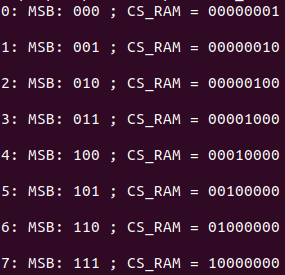
\includegraphics[width=\textwidth]{decoder_entry_3_out.png}
	\end{subfigure}
	\caption{Tableau d'entrées/sorties du décodeur pour 2 et 3 bits de poids fort en entrée}
	\label{fig:stdout_decoder_2_3}
\end{figure}


\begin{figure}[h]
	\centering
	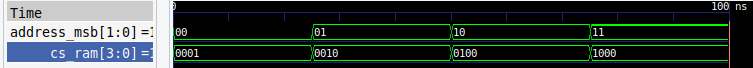
\includegraphics[width=0.97\linewidth]{decoder_entry_2_wave.png}
	\caption{Simulation du décodeur pour 2 bits de poids fort en entrée}
	\label{fig:wave_bloc_decoder}
\end{figure}

\newpage

\subsection{Bloc Quad-ram}

\indent Le bloc Quadram est le top module du bloc mémoire.
Il ne contient en réalité que des générations d'instances de RAM et du décodeur, toujours d'une façon générique suivant la taille du bus d'adresse et du bus de données.
Il n'est pas possible de déterminer manuellement le nombre de blocs RAM instancié, celui-ci est en effet calculé suivant le nombre de bits de poids forts pris en compte : pour n-bits, il y aura $ 2^{n} $ cellules RAM. Cette implémentation est choisie car calculer un log de 2 avec des composants matériels rajoutent une complexité non souhaitée à l'application.

\begin{figure}[h]
	\centering
	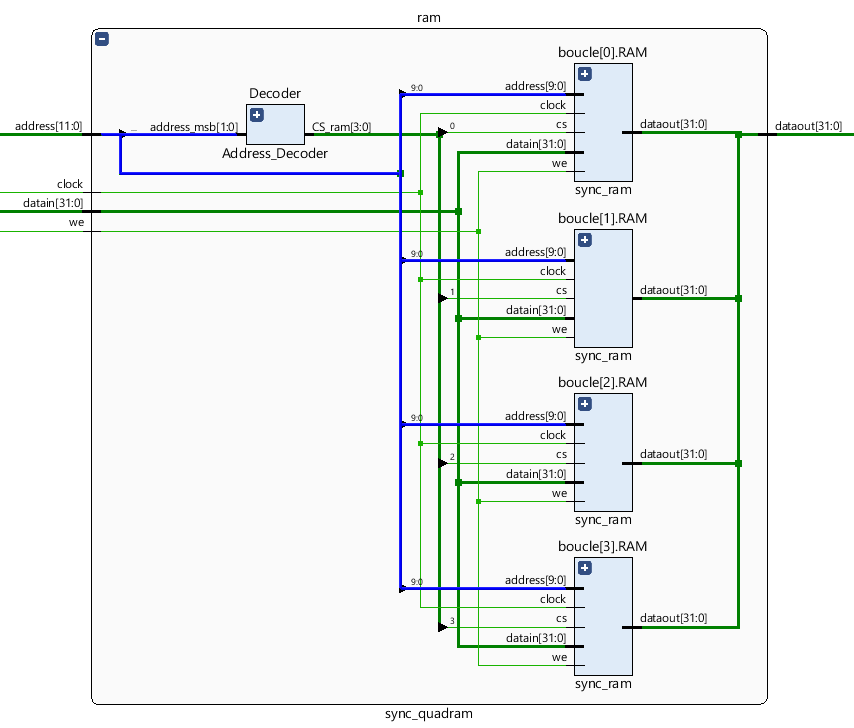
\includegraphics[width=0.97\linewidth]{bloc_quadram.png}
	\caption{Bloc mémoire complet niveau RTL}
	\label{fig:synth_bloc_quadram}
\end{figure}

\indent Le décodeur prend en entrée un nombre spécifié en paramètres de bits; ici, 2 bits en entrée. 
Il y a donc un bus \textit{CS\_ram} en sortie qui est décomposé vers 4 cellules RAM. 
Le reste des bits du bus d'adresses ainsi que le bus de données sont en entrées des cellules RAM.
Nous avons donc pu générer un banc de tests avec Cocotb qui consiste à faire un cycle de 5 écritures à des adresses aléatoires en mémoire puis de faire 5 cycles de lecture à ces mêmes adresses pour vérifier le contenu des blocs RAM et le fonctionnement des signaux \textit{Chip Select}.

\newpage

\begin{figure}[h]
	\centering
	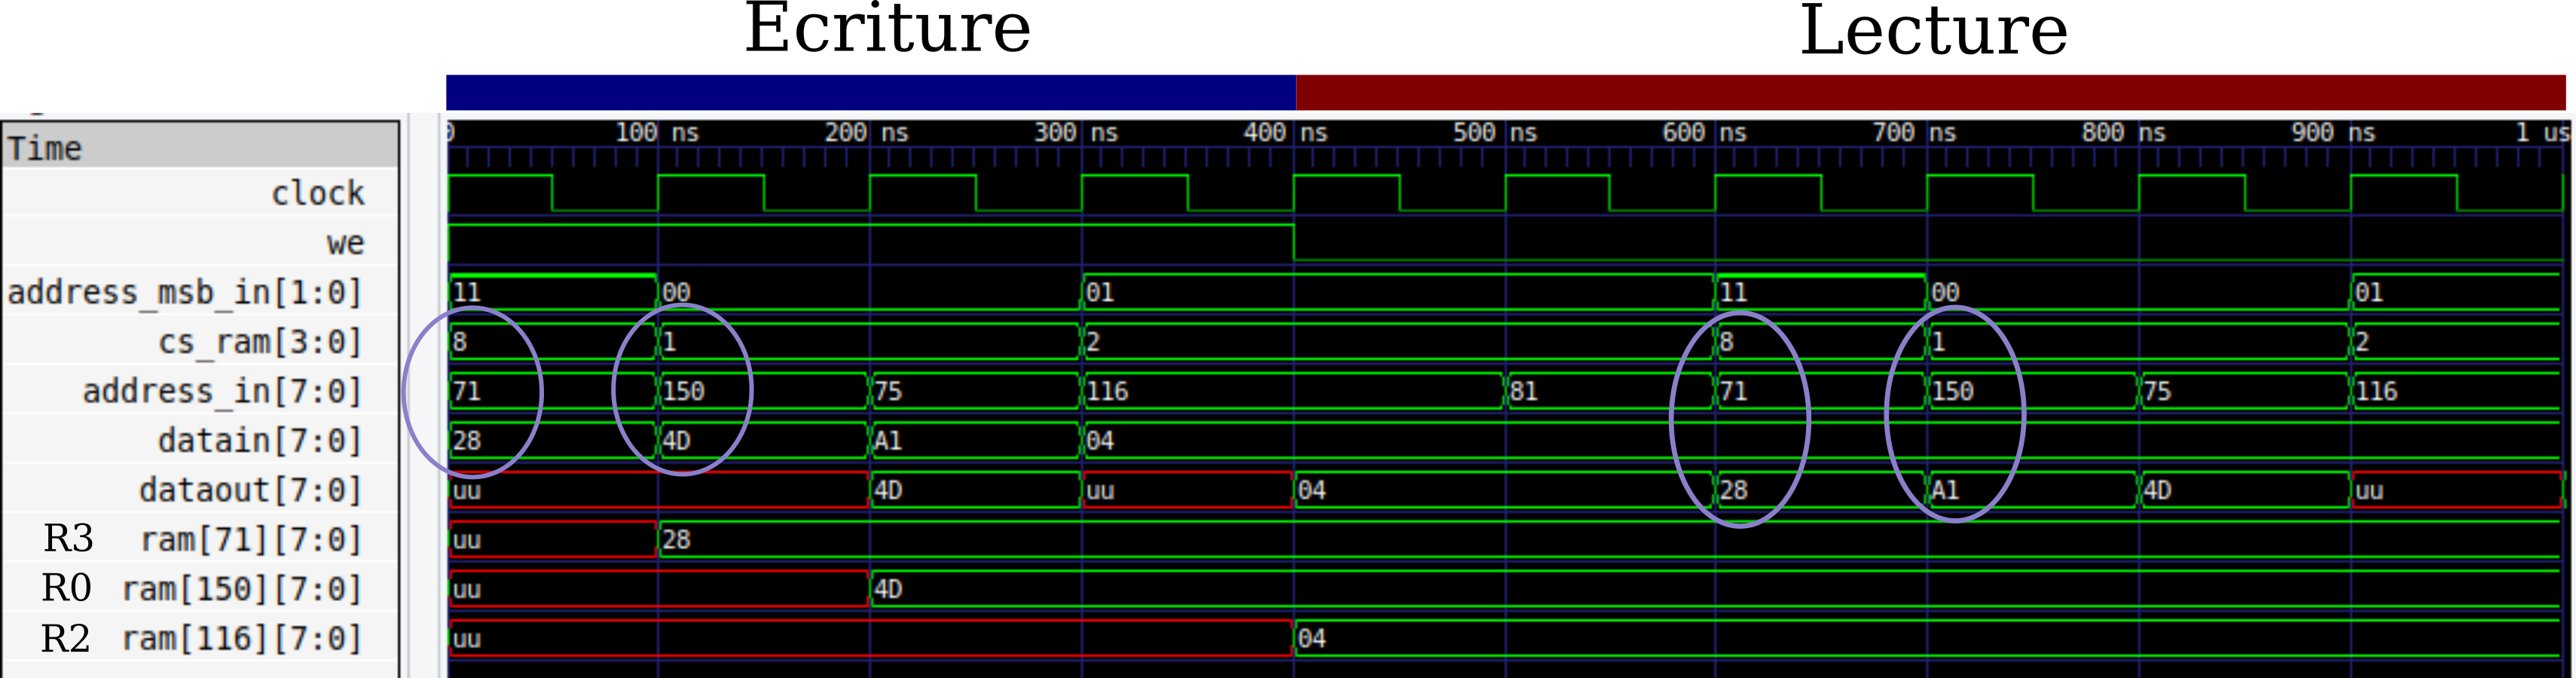
\includegraphics[width=0.97\linewidth]{quadram_wave.draw.png}
	\caption{Simulation du bloc mémoire complet}
	\label{fig:wave_bloc_quadram}
\end{figure}

\indent Comme pour tester le comportement d'une cellule RAM, 5 cycles d'écritures sont effectués puis 5 cycles de lecture.
Sur la figure ci-dessus, les valeurs contenues aux adresses des RAMs correspondent à l'écriture qui a eu lieu au cycle d'horloge précédent.
Pour les lecture, le bon fonctionnement est moins évident puisqu'en effet, à 700 ns, la valeur lue à l'adresse 150 de la RAM0 n'est pas 4D comme attendu, mais A1; ceci est dû à la sauvegarde de \textit{read\_address} qui lors de la dernière activation de la RAM0, avait pour valeur 75.
Ainsi, au cycle d'horloge suivant la valeur 4D est lue à l'adresse de lecture 150.
Ce cycle d'horloge supplémentaire vient de notre décision d'affecter la valeur \textit{address} à \textit{read\_address} uniquement lorsque le signal \textit{cs} est à l'état haut; nous trouvions illogique d'avoir une affectation permanente alors que les adresses peuvent être destinées qu'à une seule RAM à chaque cycle.
Les valeurs indéfinies sur le bus de sortie correspondent à une lecture à une adresse où aucune valeur n'a été écrite. \\

\indent Le nom donné par défaut au bloc est "Quadram" mais en réalité le modèle pourrait en contenir 1, 2, 8, 16 ...

